% Kopfzeile beim Kapitelanfang:
\fancypagestyle{plain}{
%Kopfzeile links bzw. innen
\fancyhead[L]{\calligra\Large Vorlesung Nr. 17}
%Kopfzeile rechts bzw. außen
\fancyhead[R]{\calligra\Large 06.12.2012}
}
%Kopfzeile links bzw. innen
\fancyhead[L]{\calligra\Large Vorlesung Nr. 17}
%Kopfzeile rechts bzw. außen
\fancyhead[R]{\calligra\Large 06.12.2012}
% **************************************************
\wdh
\begin{itemize}
\item{Komplexe Exponentialfunktion: $exp:\C→\C,\ z\mapsto exp(z)\ds \sum_{n\geq 0}\frac{z^n}{n!}$ stetig, Funktionalgleichung: $e^{z+w}=e^z·e^w, z,w\eC$
Additionstheoreme: $cos(x+y)=Re(e^{i(x+y)})=Re(e^{i(x)}·e^{i(y)})=cos(x)·cos(y)-sin(x)·sin(y)$}
\item{Sinus, Cosinus: $sin,cos:\R→\R,\ sin(x):=Im(e^{ix}),\ cos(x):=Re(e^{ix}),\ e^{ix}=cos(x)+i·sin(x)$}
\item{Weil $exp:\C→\C$ stetig \Rarr\ $sin, cos:\R→\R$ stetig
\usetikzlibrary{decorations.pathreplacing}
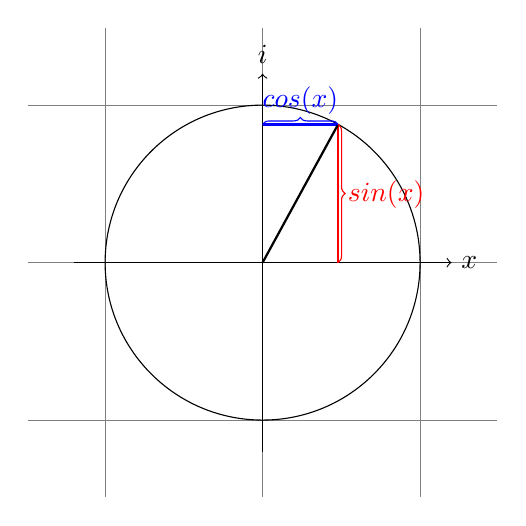
\begin{tikzpicture}[domain=-1.2:1.2, scale=2]
    \draw[very thin,color=gray] (-1.49,-1.49) grid (1.49,1.49);
    \draw[->] (-1.2,0) -- (1.2,0) node[right] {$x$};
    \draw[->] (0,-1.2) -- (0,1.2) node[above] {$i$};
	\draw (0,0) circle (1cm);
	\draw[thick, blue](0,0.8775) -- (0.4794, 0.8775);
	\draw[thick, red](0.4794,0) -- (0.4794, 0.8775);
	\draw[thick, black](0,0) -- (0.4794, 0.8775);
	\draw[decorate,decoration=brace,red] (0.4794, 0.8775) -- (0.4794,0);
	\draw[decorate,decoration=brace,blue] (0,0.8775) -- (0.4794, 0.8775);
	\draw (0.4794, 0.43) node[right, red] {$sin(x)$};
	\draw (0.24, 0.8775) node[above, blue] {$cos(x)$};
\end{tikzpicture}
\desc{Problem: zu zeigen}{$\~{sin}$ und $sin$ aus Vorlesung\\*
$\~{cos}$ und $cos$ aus Vorlesung}
\tikz[scale=2,domain=-0.49:2.5, samples=200,prefix=plots/,smooth]{
      \draw[very thin, color=gray!50] (-0.49,-0.25) grid (2.49,2.49);
      \draw[->] (-0.5,0) -- (2.5,0) node[right] {$x$};
      \draw[->] (0,-0.5) -- (0,2.5) node[above] {$y$};
      \clip (-0.49,-0.5) rectangle (2.5,2.5);
      \draw[color=red] plot[id=x] function{x} node[below]{\footnotesize $f_1(x) =x$};
      \draw[color=blue] plot[id=abs,sharp plot] function{sin(x)} node {\footnotesize $f_2(x) = sin(x)$};
      \draw[color=cyan] plot[id=x3d6] function{x - (x**3 / 6)} node [below] {\footnotesize $f_2(x) = x - \frac{x^3}{6}$};
}
}
\end{itemize}
Potenzreihen von $sin$ und $cos$:
Für $x \in \R$ gilt:
$$cos(x) + i \cdot sin(x) = exp(i \cdot x) = \frac{1}{0!}+\frac{i \cdot x}+{1!}+\frac{(i \cdot x)^2}{1!}+{2!}+\frac{(i \cdot x)^3}{3!}+…$$
$$=(\frac{1}{0!} + \frac{(i \cdot x)^2}{2!} + \frac{(i \cdot x)^4}{4!}) + \frac{(i \cdot x)^6}{6!} + …) + i (\frac{(i \cdot x)}{1!} + \frac{(i \cdot x)^3}{3!}) + \frac{(i \cdot x)^5}{5!}) + …)$$
\sS{Satz}
Für $x \in R$ gilt:
$$cos(x) = \ds\sum_{k \geq 0} \frac{(-1)^k}{(2k)!} \cdot x^{2k},\ sin(x) =\sum_{k \geq 0} \frac{(-1)^k}{(2k +1)!} \cdot x^{2k+1} $$
\sS{Bemerkung}
Siehe Übung\\*
$$cos(x)-cos(y)=2sin \ldots$$

% Satz 7.26


\uS{Analytische Definition der Zahl \pi}
\sS{Lemma}
Für $0<x\leq 2$ gilt: $0<x-\frac{x^3}{6}<sin(x)<x$.\\*
\begin{tikzpicture}[domain=-2:7,prefix=plots/, smooth]
    \draw[very thin,color=gray] (-2,-1.2) grid (7,1.2);
    \draw[->] (-2,0) -- (7,0) node[right] {$x$};
    \draw[->] (0,-1.2) -- (0,1.2) node[above] {$i$};
	\draw[color=red] plot[id=sin1] function{sin(x)} node[above, pos=0.5] {\footnotesize $f_1(x) = sin(x)$};
	\draw[color=blue] plot[id=cos1] function{cos(x)} node[below, midway] {\footnotesize $f_2(x) = cos(x)$};
\end{tikzpicture}

\bew
Schreibe $sin(x)=\sum(-1)^na_n$ mit $a_n\dfrac{x^{2n+1}}{(2n+1)!}>0$\\*[4pt]
Für $n\geq 1$ gilt: $$\frac{a_{n+1}}{a_n}=\dfrac{x^{2(n+1)+1}}{(2(n+1)+1)!}·\dfrac{(2n+1)!}{x^{2n+1}}=\frac{x^2}{(2n+3)·(2n+2)}<1$$
also: $a_1>a_2>a_3>a_4>…$\\*
Damit: $$x-sin(x)=\underset{>0}{(a_1-a_2)}+\underset{>0}{(a_3-a_4)}+\underset{>0}{(a_5-a_6)}…>0,\text{ d.h. $sin(x)<x$}$$
$$sin(x)-(x-\frac{x^3}{6})=\underset{>0}{(a_2-a_3)}+\underset{>0}{(a_4-a_5)}…>0,\text{ d.h. $sin(x)>x-\frac{x^3}{6}$}$$
Schließlich gilt für $0<x\leq 2$:
$$0<x-\frac{x^3}{6}, \text{ denn } \frac{x^3}{6}=\frac{x·x^2}{6}\leq x·\frac{4}{6}<x$$ \qed

\subsection*{Lemma} es gilt $cos(2) < 0$ und $cos(1) > 0$
\bew
	Es gilt $cos(2) = \sum (-1)^n \cdot b_n$, $b_n = \frac{2^{2n}}{(2n)!}$. Für $n \geq 1$ gilt: 
	$$\frac{b_{n+1}}{b_n} = \frac{2^2}{(2n+1)(2n+2)} < 1$$
	Also $b_1 > b_2 > b_3 > b_4 >…$ \\*[8pt]
	Somit:\\
	$cos(2) = b_0 - b_1 + b_2 - b_3 + b_4 - …$\\*
	$= b_0 - b_1 + b_2 \underbrace{-(b_3 + b_4)}_{<0} \underbrace{-(b_5 + b_6)}_{< 0}… < b_0 - b_1 + b_2$ \\*
	$= 1 - 2 + \frac{2}{3} = - \frac{1}{3}$ \qed\\
	Analog $cos(1) > 1-\frac{1}{2}$

\sS{Lemma}
Die Funktion $cos:[0,2]→\R$ ist streng monoton fallend im Intervall\\*
 \tikz[scale=2,domain=-0.49:2.5, samples=200,prefix=plots/,smooth]{
      \draw[very thin, color=gray!50] (-0.2,-0.25) grid (2,1.2);
      \draw[->] (-0.5,0) -- (2,0) node[right] {$x$};
      \draw[->] (0,-0.5) -- (0,1.2) node[above] {$y$};
      \draw[color=red] plot[id=x] function{x/1.4} node[below]{\footnotesize $cos$};
      \draw[color=red] plot[id=x] function{1 - x/(1.4)} node[below]{\footnotesize $sin$};
}
\bew
Sei $2\geq x>x\geq 0$, dann gilt $cos(x)-cos(y)\underset{\overset{\uparrow}{Additionstheoreme}}{=}-2·sin(\frac{x+y}{2})·sin(\frac{x-y}{2})$\\*
Weil $\frac{x+y}{2}, \frac{x-y}{2}\in (0,2]$ gilt mit Lemma 7.27\\*
$cos(x)-cos(y)<0$, d.h. $cos(x)<cos(y)\qed$

\sS{Satz}
Die Funktion $cos:[0,2]→\R$ hat genau eine Nullstelle $x$, und es gilt $x>1$
\bew
\begin{itemize}
\item{$cos(1)>0,\ cos(2)<0,\ cos$ stetig $\underset{Zwischenwertsatz}{\Rarr}\ cos$ \ul{hat} Nullstelle $x\in(1,2)\ (1<x<2)$}
\item{Da $cos:[0,2]→\R$ streng monoton fallend, hat $cos$ \ul{genau} eine Nullstelle \qed}
\end{itemize}

\sS{Definition}
Es sei $\pi\eR$ die eindeutige Zahl, so dass $cos(\frac{\pi}{2})$ und $1\leq\frac{\pi}{2}\leq 2$
\bem
$2\leq \pi \leq 4$, tatsächlich: $\pi=3,14159…$ (Kreiszahl)
\ul{es gilt}
Es gilt:\\*
\begin{tabular}{l|c|c|c|c|c|l}
$x$ & $0$ & $\frac{\pi}{2}$ & $\pi$ & $\frac{3 \cdot \pi}{2}$ &\\\hline
$cos(x)$ & $1$ & $0$ & $-1$ & $0$ & $1$ & \\\hline
$sin(x)$ & $0$ & $1$ & $0$ & $-1$ & $0$ & \\\hline
\end{tabular}
\hfill\\*
dazu:
\begin{enumerate}
\item{$sin(x)^2 + cos(x)^2 = 1$\\*
$sin(\frac{\pi}{2})^2 = 1$ also $sin(\frac{\pi}{2} = \pm 1$ aber $sin(\frac{\pi}{2}) > 0$\\*
d.h.:\\*
$e^{i \frac{\pi}{2}} = cos(\frac{\pi}{2}) + i \cdot sin(\frac{\pi}{2}) = i$}
\item{$$e^{i\cdot \pi} = (e^{i\cdot \frac{\pi}{2}})^2 = i^2 = -1 = cos(\pi) + i \cdot sin(\pi)$$}
\item{$$e^{i\frac{3 \cdot \pi}{2}} = e^{i\pi} \cdot e^{i\frac{\pi}{2}} = -1 \cdot i = -i = cos(\frac{3\pi}{2}) + i \cdot sin(\frac{3\pi}{2})$$}
\item{…}
\end{enumerate}

\sS{Satz}
Für $x\eR$ gilt:\\*
\begin{enumerate}
\item{$\ds cos(2\pi+x)=cos(x),\ sin(2\pi+x)=sin(x)$}
\item{$\ds cos(\pi+x)=-cos(x),\ sin(\pi+x)=-sin(x)$}
\item{$\ds cos(\pi-x)=cos(-x)=-cos(x),\ sin(\pi-x)=sin(x)$}
\item{$\ds cos(\frac{\pi}{2}-x)=sin(x)$}
\end{enumerate}
\Bew{Additionstheoreme anwenden}
\begin{enumerate}
\item{$\ds cos(2\pi+x)=\underset{=1}{cos(2\pi)}·cos(x)-\underset{=0}{sin(2\pi)}·sin(x)=cos(x)$}
\setcounter{enumi}{3}
\item{$\ds cos(\frac{\pi}{2}-x)=\underset{=0}{cos(\frac{\pi}{2})}·cos(-x)-\underset{=1}{sin(\frac{\pi}{2})}·\underset{=-sin(x)}{sin(-x)}=sin(x)$}
\end{enumerate}
\bem
$cos,sin$ sind periodisch mit Periode $2\pi$, $sin,cos$ sind durch $cos:[0,\frac{\pi}{2}]→\R$ eindeutig bestimmt.
\bem
$cos(x),sin(x)$ kann für $x\in \{0,\frac{\pi}{6},\frac{\pi}{4},\frac{\pi}{3},\frac{\pi}{2}\}$ explizit bestimmt werden
\bsp
$cos(\frac{\pi}{3})=\frac{1}{2},\ sin(\frac{\pi}{3})=\frac{\sqrt{3}}{2}$
\bew
	Sei $x = cos (\frac{\pi}{3}),\ y = sin(\frac{\pi}{3}), z = x + i\cdot y = e^{i\frac{\pi}{3}}$\\*
	Dann gilt:\\*
	$$z^2 = e^{2 \cdot i\frac{\pi}{3}} = e^{i\pi \cdot - \frac{\pi}{3}} = -1 \cdot e^{i\frac{\pi}{3}} = -\bar{z}$$\\*
	Also $(x + iy)^2 = -x + iy$ d.h. $x^2 - y^2 = -x$, $2xy = y$ und $x^2 + y^2 = 1$\\*
	Auflösen liefert Beh.